% Inside one Qwen3-0.6B attention sublayer (bottom -> top). Shapes per sequence (batch omitted).
\documentclass[border=8pt]{standalone}
% Shared TikZ style for every figure in "Post-training LLMs with RL" (see ../STYLE.md).
% Visual grammar follows the FME office-hours house style; the one accent colour is fern green.
% Compile with XeLaTeX, two passes (annotated equations remember node positions).
\usepackage{fontspec}
\setmainfont{Avenir Next}[BoldFont={Avenir Next Demi Bold}, ItalicFont={Avenir Next Italic}]
\setsansfont{Avenir Next}[BoldFont={Avenir Next Demi Bold}, ItalicFont={Avenir Next Italic}]
\renewcommand{\familydefault}{\sfdefault}
\hyphenpenalty=10000 \exhyphenpenalty=10000 % no hyphenation in notes and labels
\usepackage{amsmath,amssymb}
\usepackage{tikz}
\usetikzlibrary{arrows.meta,positioning,calc,fit,backgrounds,shapes.geometric,decorations.pathreplacing}

% ---------------- palette ----------------
\definecolor{ink}{HTML}{111111}
\definecolor{grey700}{HTML}{4A4F55}
\definecolor{grey500}{HTML}{6B7178}
\definecolor{grey400}{HTML}{8A9097}
\definecolor{grey300}{HTML}{D5D9DD}
\definecolor{grey100}{HTML}{F4F5F6}
\definecolor{fern}{HTML}{4F7942}       % the one accent: what the figure is about
\definecolor{ferndark}{HTML}{2F4A28}
\definecolor{fernlight}{HTML}{B5CFA8}
\definecolor{ferntint}{HTML}{EAF1E6}
% aliases used by older figure files
\colorlet{gray7}{grey700}\colorlet{gray5}{grey500}\colorlet{gray3}{grey300}\colorlet{gray1}{grey100}

% ---------------- visual grammar ----------------
\tikzset{
  every picture/.style={line cap=round, line join=round, color=ink},
  tensor/.style={draw=ink, line width=0.8pt, fill=white},
  param/.style={draw=grey700, line width=0.8pt, fill=grey100},
  op/.style={draw=grey500, line width=0.8pt, rounded corners=3pt, fill=white, inner sep=4pt, font=\small},
  accent/.style={draw=fern, line width=1.2pt},
  flow/.style={-{Stealth[length=5pt]}, line width=0.8pt, draw=grey700},
  flowa/.style={flow, draw=fern},
  tname/.style={font=\normalsize, text=ink},
  dims/.style={font=\footnotesize, text=grey500},
  note/.style={font=\footnotesize, text=grey700, align=left},
  accentnote/.style={font=\footnotesize, text=fern, align=left},
  lead/.style={draw=grey400, line width=0.5pt},
  stream/.style={draw=grey300, line width=5pt},
  block/.style={draw=grey500, line width=0.8pt, rounded corners=4pt, fill=white, align=center, font=\small, minimum height=0.8cm},
  blocka/.style={block, accent, fill=ferntint},
  frozen/.style={block, fill=grey100},
  plus/.style={circle, draw=grey700, line width=0.8pt, fill=white, inner sep=0pt, minimum size=0.42cm, font=\small},
  junction/.style={circle, fill=grey700, inner sep=0pt, minimum size=4pt},
  wire/.style={line width=0.8pt, draw=grey700},
}

% ---------------- numbered annotation system ----------------
%   markers on the drawing:  \mk{(x,y)}{1}   \mka{(x,y)}{2} (accent)
%   notes column:            \notesat{(x,y)}{width}  then  \note{1}{text}  /  \notea{2}{text}
%   symbols strip:           \symbols{$x$ & prompt \\ $y$ & response}
\tikzset{
  marker/.style={circle, fill=grey700, text=white, font=\footnotesize\bfseries, inner sep=0pt, minimum size=0.46cm},
  markera/.style={marker, fill=fern},
}
\newcommand{\mk}[2]{\node[marker] at #1 {#2}}
\newcommand{\mka}[2]{\node[markera] at #1 {#2}}
\newlength{\notewidth}
\newcommand{\notesat}[2]{%
  \node[inner sep=0pt, minimum size=0pt, anchor=north west] (note0) at #1 {};
  \setlength{\notewidth}{#2}\xdef\lastnote{note0}}
\newcommand{\note}[2]{%
  \node[font=\small, text=ink, align=left, text width=\notewidth, anchor=north west, inner sep=0pt] (note#1) at ($(\lastnote.south west)+(0.55cm,-0.32cm)$) {#2};
  \node[marker] at ($(note#1.north west)+(-0.30cm,-0.15cm)$) {#1};
  \path (note#1.south west) ++(-0.55cm,0) node[inner sep=0pt, minimum size=0pt] (note#1base) {};
  \xdef\lastnote{note#1base}}
\newcommand{\notea}[2]{%
  \node[font=\small, text=ferndark, align=left, text width=\notewidth, anchor=north west, inner sep=0pt] (note#1) at ($(\lastnote.south west)+(0.55cm,-0.32cm)$) {#2};
  \node[markera] at ($(note#1.north west)+(-0.30cm,-0.15cm)$) {#1};
  \path (note#1.south west) ++(-0.55cm,0) node[inner sep=0pt, minimum size=0pt] (note#1base) {};
  \xdef\lastnote{note#1base}}
\newcommand{\symbols}[1]{%
  \node[anchor=north west, inner sep=0pt, align=left, font=\small, text=grey700] (symbols)
    at ($(\lastnote.south west)+(0,-0.75cm)$)
    {\textcolor{grey400}{\scriptsize\bfseries SYMBOLS}\\[3pt]
     \begin{tabular}{@{}l@{\hspace{8pt}}l@{}}#1\end{tabular}};
  \draw[grey300, line width=0.5pt] ($(symbols.north west)+(0,0.18cm)$) -- ++(\notewidth+0.55cm,0);}

% ---------------- glyphs ----------------
\tikzset{
  expand/.style={draw=grey700, line width=0.8pt, fill=grey100, trapezium, trapezium stretches body,
                 trapezium left angle=64, trapezium right angle=64, shape border rotate=180,
                 minimum height=0.72cm, align=center, font=\small, inner xsep=2pt},
  contract/.style={expand, shape border rotate=0},
  silubox/.style={block, path picture={
      \begin{scope}[sharp corners, shift={($(path picture bounding box.west)+(0.45,-0.05)$)}, x=0.1cm, y=0.1cm]
        \draw[grey300, line width=0.4pt] (-3,0) -- (2.6,0);
        \draw[grey500, line width=1pt, domain=-3:2.4, samples=30] plot (\x, {\x/(1+exp(-\x))});
      \end{scope}}},
}

% ---------------- annotated equations (arrow + plain-language label per term) ----------------
% \tm{name}{math}: wrap one term of a formula in a named node. Put the formula node at (0,0)
% with anchor=base west, otherwise the remembered positions are offset.
\newcommand{\tm}[2]{\tikz[remember picture,baseline=(#1.base)]{\node[inner sep=1pt,outer sep=0pt] (#1) {$\displaystyle #2$};}}
\tikzset{
  lbl/.style   = {font=\large, text=ferndark, align=left, inner sep=2pt},
  lblg/.style  = {lbl, text=grey700},
  arr/.style   = {-{Stealth[length=8pt,width=6pt]}, line width=1.0pt, draw=fern, shorten >=3pt},
  arrg/.style  = {arr, draw=grey500},
  brc/.style   = {decorate, decoration={brace, mirror, amplitude=9pt, raise=5pt}, line width=1.4pt},
  % older diagram styles (kept for existing figures)
  blk/.style   = {draw=grey500, line width=0.9pt, rounded corners=6pt, fill=white, align=center, inner sep=7pt, minimum height=11mm, text=ink},
  blkf/.style  = {blk, draw=fern, line width=1.2pt, fill=ferntint},
  blkg/.style  = {blk, fill=grey100},
  ar/.style    = {-{Stealth[length=7pt,width=5pt]}, line width=1.0pt, draw=grey700},
  arf/.style   = {ar, draw=fern},
  capt/.style  = {font=\normalsize, text=grey500, align=center},
}

% ---------------- annotation protocol for equations ----------------
% The formula is one node named "eq" at (0,0), anchor=base west. Terms are wrapped with \tm.
% Labels sit in fixed rows ABOVE (a) or BELOW (b) the formula, tier 1 (near) or 2 (far), centred on
% their term (optional x-nudge), joined by a straight vertical leader with a dot on the term.
% No curved arrows, no diagonals. Tier-1 labels are at most two lines; tier-2 leaders pass between
% tier-1 labels. Sides l / r (outermost terms only): label beside the term, horizontal leader;
% the 4th argument is then a y-nudge.   \ann{term}{a|b|l|r}{1|2}{nudge}{text}    \anna{...} = accent (the slide's point)
\tikzset{
  annlbl/.style  = {font=\normalsize, text=grey700, align=center, inner sep=1.5pt},
  annlbla/.style = {annlbl, text=ferndark},
  annlead/.style = {draw=grey400, line width=0.6pt},
  annleada/.style= {draw=fern, line width=0.9pt},
}
\newcommand{\annrow}[2]{\ifnum#2=1 #1 0.55cm\else #1 1.95cm\fi}
\newcommand{\anngeneric}[7]{% #1 style-suffix, #2 term, #3 side, #4 tier, #5 nudge, #6 text, #7 lead style
  \if#3a
    \ifnum#4=1 \def\annoff{0.55cm}\else\def\annoff{1.95cm}\fi
    \node[annlbl#1, anchor=south] (ann-#2) at ($(#2.north |- eq.north)+(#5,\annoff)$) {#6};
    \draw[#7] ($(#2.north)+(0,0.13)$) -- (#2.north |- ann-#2.south);
    \fill[#7] ($(#2.north)+(0,0.13)$) circle (1.4pt);
  \else\if#3l
    \node[annlbl#1, anchor=east] (ann-#2) at ($(#2.west)+(-0.6cm,#5)$) {#6};
    \draw[#7] ($(#2.west)+(-0.13,0)$) -- (ann-#2.east |- {$(#2.west)+(0,0)$});
    \fill[#7] ($(#2.west)+(-0.13,0)$) circle (1.4pt);
  \else\if#3r
    \node[annlbl#1, anchor=west] (ann-#2) at ($(#2.east)+(0.6cm,#5)$) {#6};
    \draw[#7] ($(#2.east)+(0.13,0)$) -- (ann-#2.west |- {$(#2.east)+(0,0)$});
    \fill[#7] ($(#2.east)+(0.13,0)$) circle (1.4pt);
  \else
    \ifnum#4=1 \def\annoff{-0.55cm}\else\def\annoff{-1.95cm}\fi
    \node[annlbl#1, anchor=north] (ann-#2) at ($(#2.south |- eq.south)+(#5,\annoff)$) {#6};
    \draw[#7] ($(#2.south)+(0,-0.13)$) -- (#2.south |- ann-#2.north);
    \fill[#7] ($(#2.south)+(0,-0.13)$) circle (1.4pt);
  \fi\fi\fi}
\newcommand{\ann}[5]{\anngeneric{}{#1}{#2}{#3}{#4}{#5}{annlead}}
\newcommand{\anna}[5]{\anngeneric{a}{#1}{#2}{#3}{#4}{#5}{annleada}}

\begin{document}
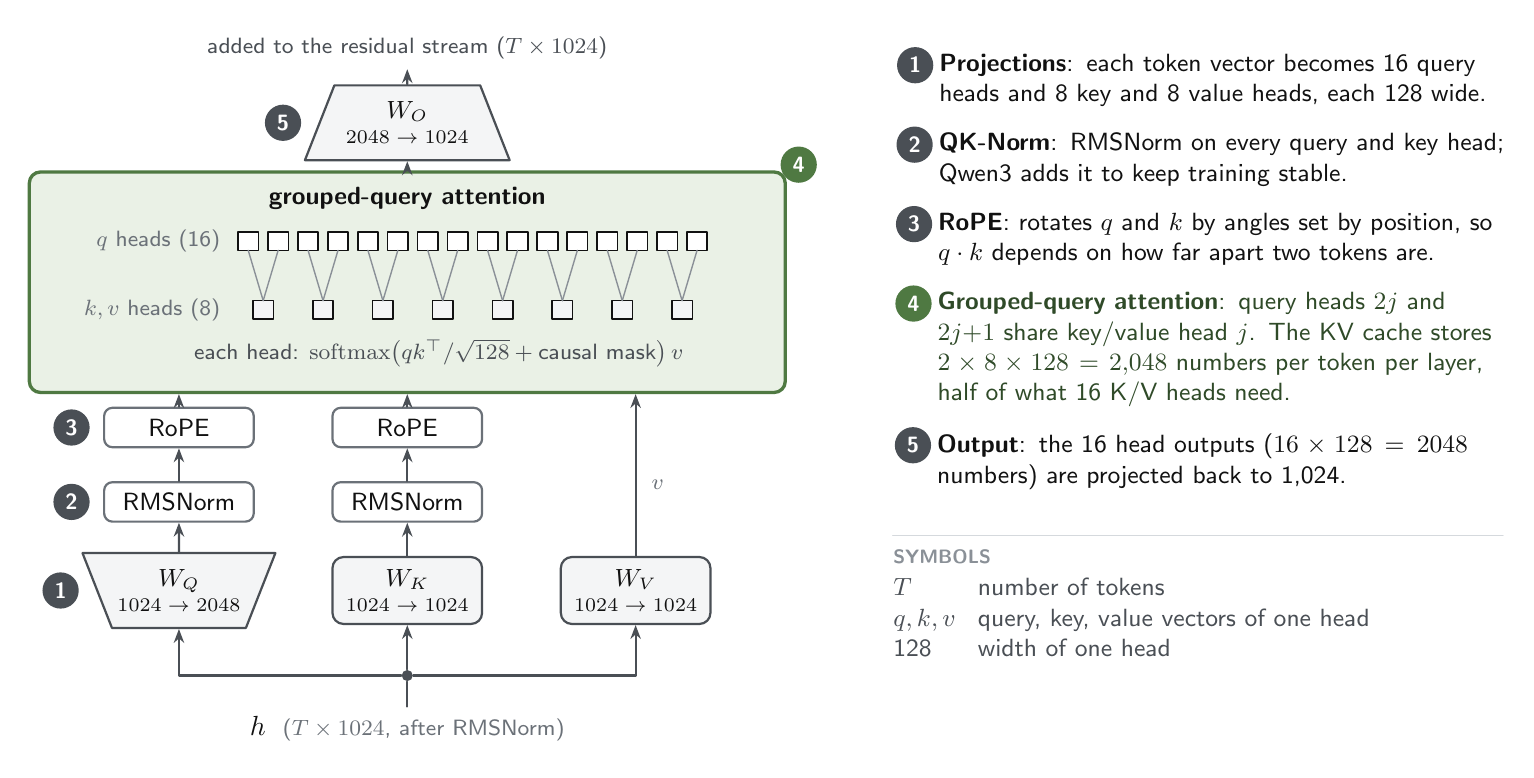
\begin{tikzpicture}[font=\small, y=0.9cm]
  \node[tname] (x) at (2.9,0) {$h$ \;\textcolor{grey500}{\footnotesize ($T\times 1024$, after RMSNorm)}};
  \node[junction] (j) at (2.9,0.75) {};
  \draw[wire] (x.north) -- (j);
  % projections, dimensions inside the glyphs
  \node[expand, minimum width=2.3cm, minimum height=0.95cm] (wq) at (0,1.95) {$W_Q$\\[-2pt]{\scriptsize $1024\to2048$}};
  \node[block, fill=grey100, draw=grey700, minimum width=1.9cm, minimum height=0.85cm] (wk) at (2.9,1.95) {$W_K$\\[-2pt]{\scriptsize $1024\to1024$}};
  \node[block, fill=grey100, draw=grey700, minimum width=1.9cm, minimum height=0.85cm] (wv) at (5.8,1.95) {$W_V$\\[-2pt]{\scriptsize $1024\to1024$}};
  \draw[flow] (j) -| (wq.south);
  \draw[flow] (j) -- (wk.south);
  \draw[flow] (j) -| (wv.south);
  % per-head RMSNorm and RoPE on q and k
  \node[op, minimum width=1.9cm] (qn) at (0,3.2) {RMSNorm};
  \node[op, minimum width=1.9cm] (kn) at (2.9,3.2) {RMSNorm};
  \node[op, minimum width=1.9cm] (qr) at (0,4.25) {RoPE};
  \node[op, minimum width=1.9cm] (kr) at (2.9,4.25) {RoPE};
  \draw[flow] (wq) -- (qn); \draw[flow] (qn) -- (qr);
  \draw[flow] (wk) -- (kn); \draw[flow] (kn) -- (kr);
  % attention block with the head-sharing icon
  \node[block, accent, fill=ferntint, minimum width=9.6cm, minimum height=2.8cm] (att) at (2.9,6.3) {};
  \node[font=\small\bfseries, text=ink, anchor=north] at ($(att.north)+(0,-0.1)$) {grouped-query attention};
  \def\xo{0.75}\def\sp{0.38}
  \foreach \i in {0,...,15} \draw[tensor, line width=0.6pt] ({\xo+\i*\sp},6.75) rectangle ++(0.26,0.26);
  \foreach \j in {0,...,7} {
    \pgfmathsetmacro{\cx}{\xo+(2*\j+0.5)*\sp+0.13}
    \draw[tensor, fill=grey100, line width=0.6pt] (\cx-0.13,5.78) rectangle ++(0.26,0.26);
    \draw[grey400, line width=0.5pt] ({\xo+(2*\j)*\sp+0.13},6.75) -- (\cx,6.04);
    \draw[grey400, line width=0.5pt] ({\xo+(2*\j+1)*\sp+0.13},6.75) -- (\cx,6.04);
  }
  \node[dims, anchor=east] at (\xo-0.1,6.88) {$q$ heads (16)};
  \node[dims, anchor=east] at (\xo-0.1,5.91) {$k,v$ heads (8)};
  \node[font=\footnotesize, text=grey700] at (3.3,5.3) {each head: $\operatorname{softmax}\!\big(q k^{\top}/\sqrt{128} + \text{causal mask}\big)\, v$};
  \draw[flow] (qr.north) -- (qr.north |- att.south);
  \draw[flow] (kr.north) -- (kr.north |- att.south);
  \draw[flow] (wv.north) -- (wv.north |- att.south);
  \node[dims, anchor=west] at ($(wv.north)+(0.08,1.0)$) {$v$};
  % output projection
  \node[contract, minimum width=2.6cm, minimum height=0.95cm] (wo) at (2.9,8.55) {$W_O$\\[-2pt]{\scriptsize $2048\to1024$}};
  \draw[flow] (att.north) -- (wo.south);
  \node[note] (out) at (2.9,9.6) {added to the residual stream ($T\times 1024$)};
  \draw[flow] (wo.north) -- (out.south);

  \mk{($(wq.west)+(-0.45,0)$)}{1};
  \mk{($(qn.west)+(-0.4,0)$)}{2};
  \mk{($(qr.west)+(-0.4,0)$)}{3};
  \mka{($(att.north east)+(0.15,0.08)$)}{4};
  \mk{($(wo.west)+(-0.45,0)$)}{5};

  \notesat{(9.1,9.9)}{7.2cm}
  \note{1}{\textbf{Projections}: each token vector becomes 16 query heads and 8 key and 8 value heads, each 128 wide.};
  \note{2}{\textbf{QK-Norm}: RMSNorm on every query and key head; Qwen3 adds it to keep training stable.};
  \note{3}{\textbf{RoPE}: rotates $q$ and $k$ by angles set by position, so $q \cdot k$ depends on how far apart two tokens are.};
  \notea{4}{\textbf{Grouped-query attention}: query heads $2j$ and $2j{+}1$ share key/value head $j$. The KV cache stores $2\times 8\times 128 = 2{,}048$ numbers per token per layer, half of what 16 K/V heads need.};
  \note{5}{\textbf{Output}: the 16 head outputs ($16\times128 = 2048$ numbers) are projected back to 1,024.};
  \symbols{$T$ & number of tokens \\ $q, k, v$ & query, key, value vectors of one head \\ 128 & width of one head};
\end{tikzpicture}
\end{document}
